\section{results}

\begin{figure}
\begin{center}
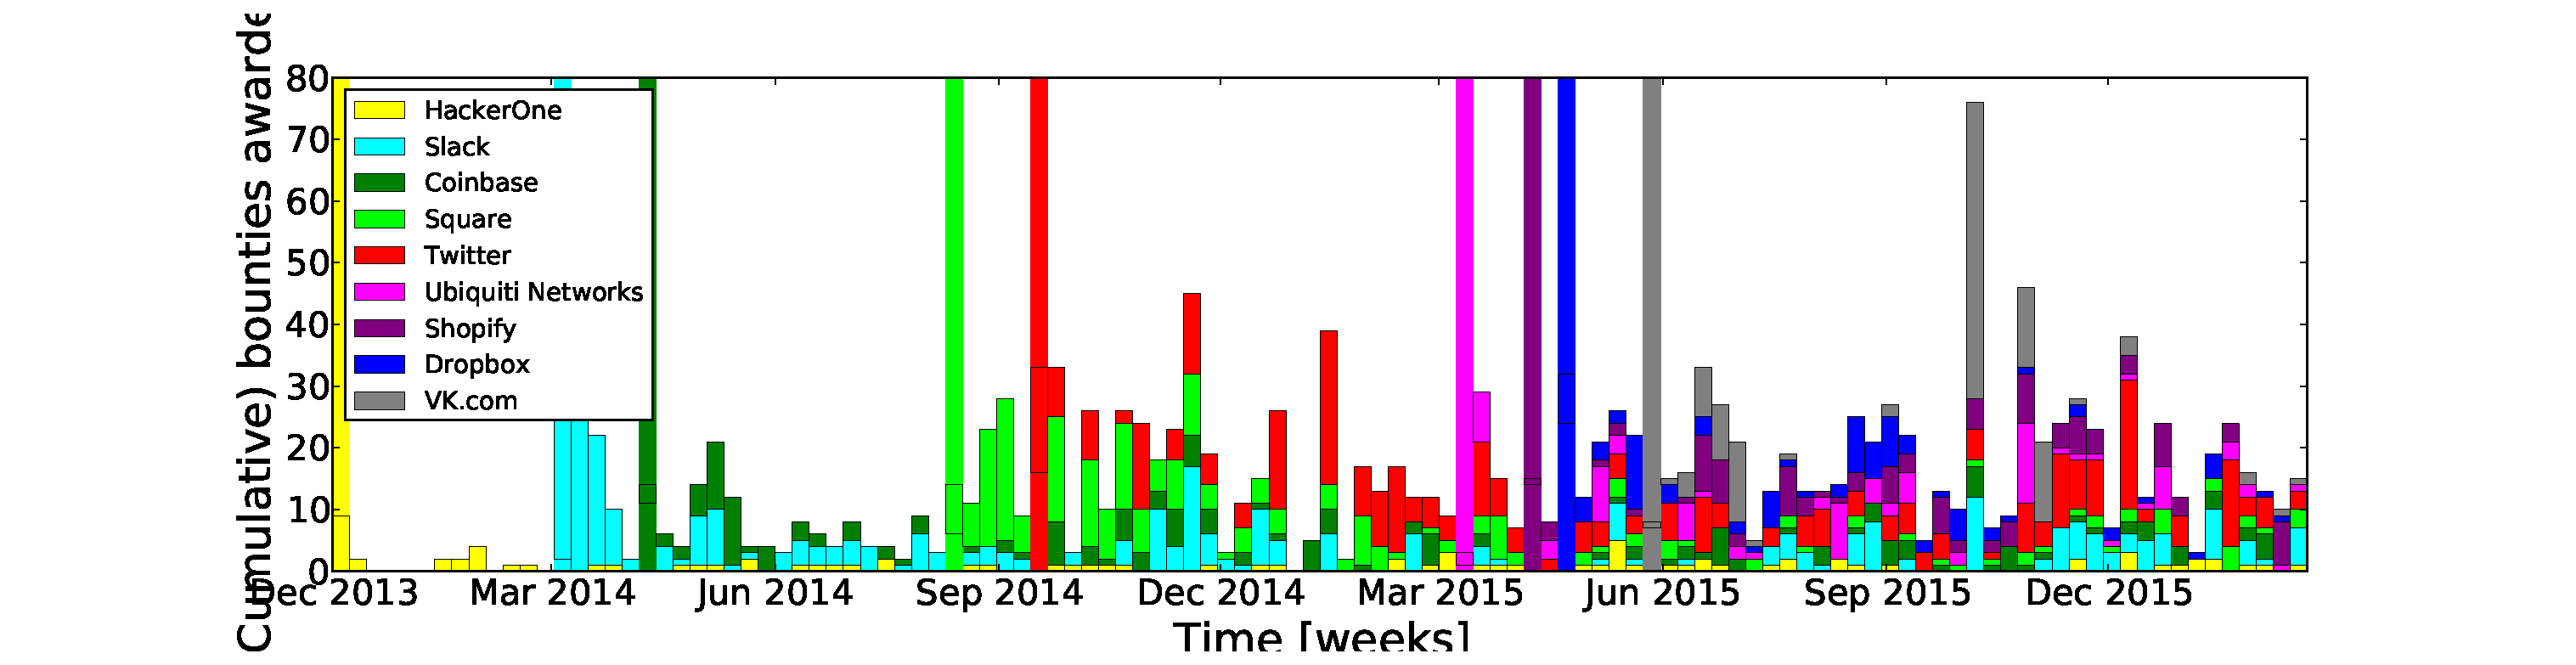
\includegraphics[width=16cm]{figures/timeline.eps}
\caption{ }
\label{ }
\end{center}
\end{figure}


\begin{figure}
\begin{center}
\includegraphics[width=10cm]{figures/density_joining.eps}
\caption{ }
\label{ }
\end{center}
\end{figure}



{\bf Scaling bugs as a function of researchers per program:}
\begin{equation}
R \sim c^{\beta}
\end{equation}

with $\beta \approx 1.13$ (see Figure \ref{fig:scaling}).


\begin{figure}
\begin{center}
\includegraphics[width=10cm]{figures/scaling_bugs_vs_researchers.eps}
\caption{ }
\label{fig:scaling}
\end{center}
\end{figure}





Let us call $\{R_1, R_2, ..., R_{c-1}, R_c\}$, the total number of bugs found respectively by security researchers $1, 2, ..., c-1, c$. 
Let us call $R_{\rm max}(c)$, the largest among the set  $\{R_1, R_2, ..., R_{c-1}, R_c\}$. A good estimate of $R_{\rm max}(c)$ is obtained by the condition that the probability $\int_{R_{\rm max}(c)}^{+\infty}  p(r) dr$ to find a security researcher with a total contribution equal to or larger than $R_{\rm max}(c)$ times the number $c$ of active developers is equal to $1$, i.e., by the definition of $R_{\rm max}(c)$, there should be typically only one 
security researcher with such a number of bugs found. This yields
\be
 R_{\rm max}(c)  \sim c^{1/\mu} ~. 
 \label{sdfjhsg9e}
\ee



An estimate of the typical total number of bugs  $R_1 +  R_2 + ... + R_c$  identified
by the $c$ security researchers can  then be obtained as  \cite{Bougeorges,sornette2006critical}
\be
R_1 +  R_2 + ... + R_c   \approx c  \int_0^{R_{\rm max}(c)} r   p(r) dr
 \sim  c^{1/\mu}    ~,~~~~{\rm  for}~\mu <1~.
 \label{rjtik6ik}
\ee


We stress that the scaling $\sim c^{1/\mu}$ only holds for $\mu <1$ and is replaced
by $\sim c$, i.e., linearity, for $\mu > 1$.
The upper bound in the integral in (\ref{rjtik6ik}) reflects that
the random variables $\{R_1, R_2, ..., R_{c-1}, R_c\}$ are not larger than $R_{\rm max}(c)$
by definition of the later. According to equation (\ref{rjtik6ik}), the typical
total production (number of commits) by $c$ developers
is proportional to $c^{1/\mu}$, when their contributions are wildly distributed
with a power law distribution with exponent $\mu <1$. According to this large
deviation mechanism, the superlinear exponent $\beta$ is equal to $1/\mu$.
\be
{\rm \bf prediction~of ~the~ large~ deviation ~mechanism}: ~\beta = 1/\mu~, ~{\rm for}~\mu < 1~.
\label{eyyn}
\ee

Within this large deviation mechanism, explaining the superlinear productive activity ($\beta>1$) 
reduces to explaining the heavy-tailed distribution of commits $R$ per contributor over a large period of time,
i.e., amounts to derive the power law distribution (\ref{srthyjueyt}) with $\mu <1$. For this, the next section
proposes a generic model.


\be
{\rm \bf prediction~of ~the~ large~ deviation ~mechanism}: ~\beta = 1/\mu~, ~{\rm for}~\mu < 1~.
\label{eyyn}
\ee


Distribution of bugs found per programmer per program:
\begin{equation}
P(X > x) = 1/x^{\alpha},~with~\gamma = 1.60(7) 
\end{equation}

{\bf Distribution of bugs per program:}
\begin{equation}
P^{tot}_{>}(R > r) = 1/x^{\mu},~with~\mu = 0.8(4) 
\end{equation}

Distribution of researchers per program:
\begin{equation}
P(X > x) = 1/x^{\gamma},~with~\alpha = 0.9(5) 
\end{equation}



{\bf mapping}

- superlinear exponent (same)\\
- bug bounty program  $\Leftrightarrow$ OSS contributor \\










\begin{figure}
\begin{center}
\includegraphics[width=16cm]{figures/ccdfs.png}
\caption{ }
\label{ }
\end{center}
\end{figure}